\clearpage
\setcounter{page}{1}
\setcounter{figure}{0}
\setcounter{table}{0}
\renewcommand{\thefigure}{S\arabic{figure}}
\renewcommand{\thetable}{S\arabic{table}}
\maketitlesupplementary

\setcounter{section}{0} % Reset section counter to 0
\renewcommand{\thesection}{S\arabic{section}} % Section 1 becomes S1
\setcounter{subsection}{0} % Reset subsection counter
\renewcommand{\thesubsection}{S\arabic{section}.\arabic{subsection}} % Sub 1.1 becomes S1.1

\section{Datasets \& Implementation Details}
\label{sec:sup_impl}
We conduct experiments on subsets of the RE10k~\cite{re10k} and DL3DV~\cite{dl3dv} datasets. For RE10k, we use approximately $6,000$ scene clips as the training split and $749$ clips as the test split. For DL3DV, we adopt its 1K-5K subsets for training, which contain roughly $5,000$ scenes, and test on the $140$ benchmark scenes.

During training, we sample 2 input views to reconstruct the aesthetic features of 12 target views in RE10k, and sample 2 to 6 input views to predict aesthetic features for 24 target views in DL3DV. We train all models for 50,000 steps with a batch size of 8. We use AdamW~\cite{loshchilov2017decoupled} with a learning rate of $0.0005$ and a cosine annealing scheduler.

\begin{figure}[h]
\centering
\begin{subfigure}[t]{0.98\linewidth}
\captionsetup{labelformat=empty}
    \centering
    \includegraphics[width=\linewidth]{figs/sup_nva_1.pdf}
    \caption{
        \textbf{Sequence 1.}
    }
    % \label{fig:sup_nva_1}
\end{subfigure}
\vfill
\begin{subfigure}[t]{0.98\linewidth}
\captionsetup{labelformat=empty}
    \centering
    \includegraphics[width=\linewidth]{figs/sup_nva_2.pdf}
    \caption{
        \textbf{Sequence 2.}
    }
    % \label{fig:sup_nva_2}
\end{subfigure}

\caption{
Additional novel view aesthetic prediction results. \textit{In both examples:} (a) Aesthetic score predictions over consecutive frames. The dashed line and box mark the regions visualized in (b) and (c), respectively.
(b) Given the same aesthetic model and viewpoint, rendering artifacts in the predicted view (\eg, wrong color prediction as marked in red boxes in \textit{top}, noisy predictions marked in blue boxes in \textit{bottom}) bias the RGB-scoring approach.  
(c) Ground-truth scores fluctuate noticeably across nearly identical nearby views. 
}
\label{fig:sup_nva}
\end{figure}

\section{Aesthetic Prediction at Novel Views}
\label{sec:sup_nva}
We provide additional qualitative examples of novel-view aesthetic prediction to further illustrate the two limitations of the RGB-based baseline approach discussed in the main paper. As shown in~\cref{fig:sup_nva}, the aesthetic model is biased by the rendering artifact, and exhibits high sensitivity to minor pixel-level variations across nearby views that are nearly identical. In contrast, our distilled aesthetic field faithfully follows the teacher's underlying trend, producing smoother and more consistent predictions across nearby frames.

\begin{figure*}[htbp]
\centering
    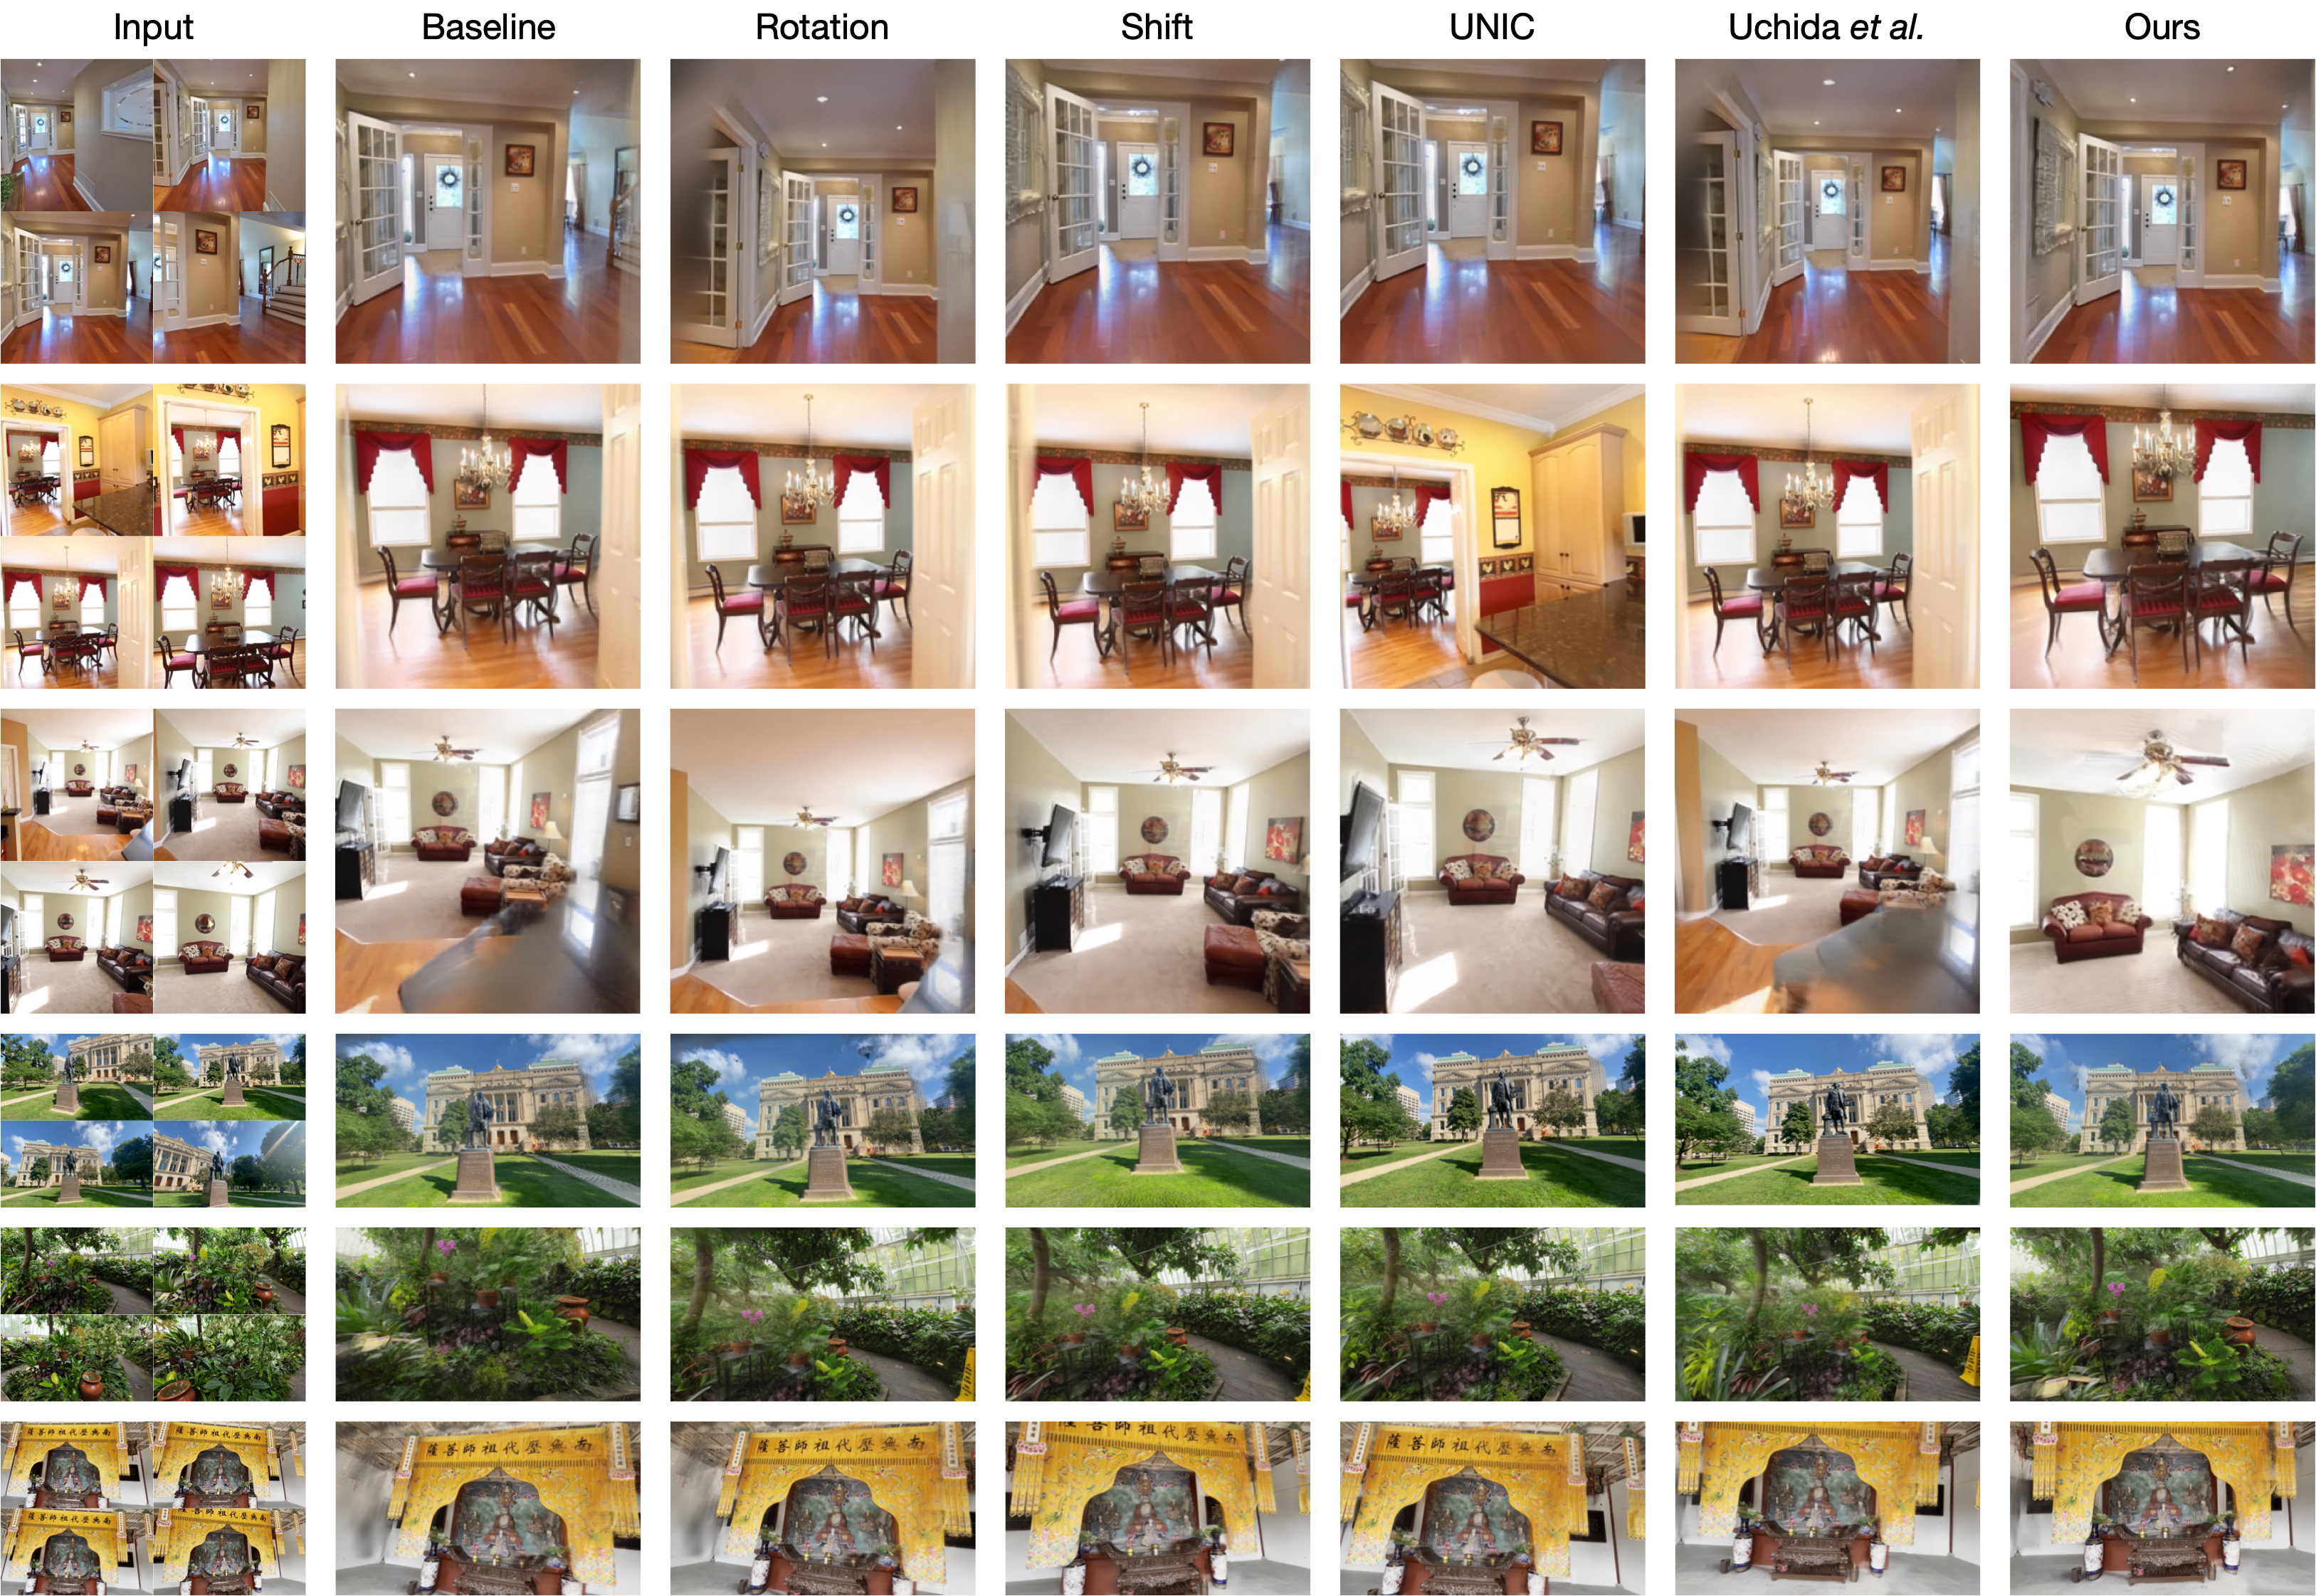
\includegraphics[width=\linewidth]{figs/sup_avs.jpg}
    \caption{Additional results of aesthetic viewpoint suggestion.}
    \label{fig:sup_avs}
\end{figure*}

\begin{figure*}[p]
\centering
    \includegraphics[width=\linewidth]{figs/sup_vis_vertical.pdf}
    \caption{Additional visualizations of sampled viewpoints colored by aesthetic score, with representative renderings shown alongside.}
    \label{fig:sup_vis}
\end{figure*}

\section{Aesthetic Viewpoint Suggestion}
\label{sec:sup_avs}
We first describe how existing single-view baselines are adapted to our evaluation setting, followed by additional qualitative comparisons of the suggested viewpoints.

UNIC~\cite{xu2023unifying} predicts crops with varying sizes in an extrapolated image plane rather than real camera motions. For fair comparison, we fix its crop size as input resolution ($256\times 256$ in RE10k and $256\times 448$ in DL3DV) and map the crop-center shifts to in-plane camera translations, thereby obtaining corresponding real viewpoints where we measure aesthetic qualities. Uchida \etal~\cite{uchida20253d} first outpaint an image, reconstruct 3D point clouds from it, and then optimize camera poses and image aspect ratios in this outpainted 3D scene. We therefore also fix their output resolution and transform their suggestions to equivalent real viewpoints for evaluation. 

As shown in~\cref{fig:sup_avs}, our method consistently suggests viewpoints with superior framing and composition than comparison methods.

Finally, additional 3D visualizations of the viewpoint sampling results are shown in~\cref{fig:sup_vis}. The results demonstrate the variation of aesthetic quality across 3D space, and the corresponding renderings confirm strong alignment between our model's evaluations and human perceptual preferences.

\begin{figure*}[t]
\centering
    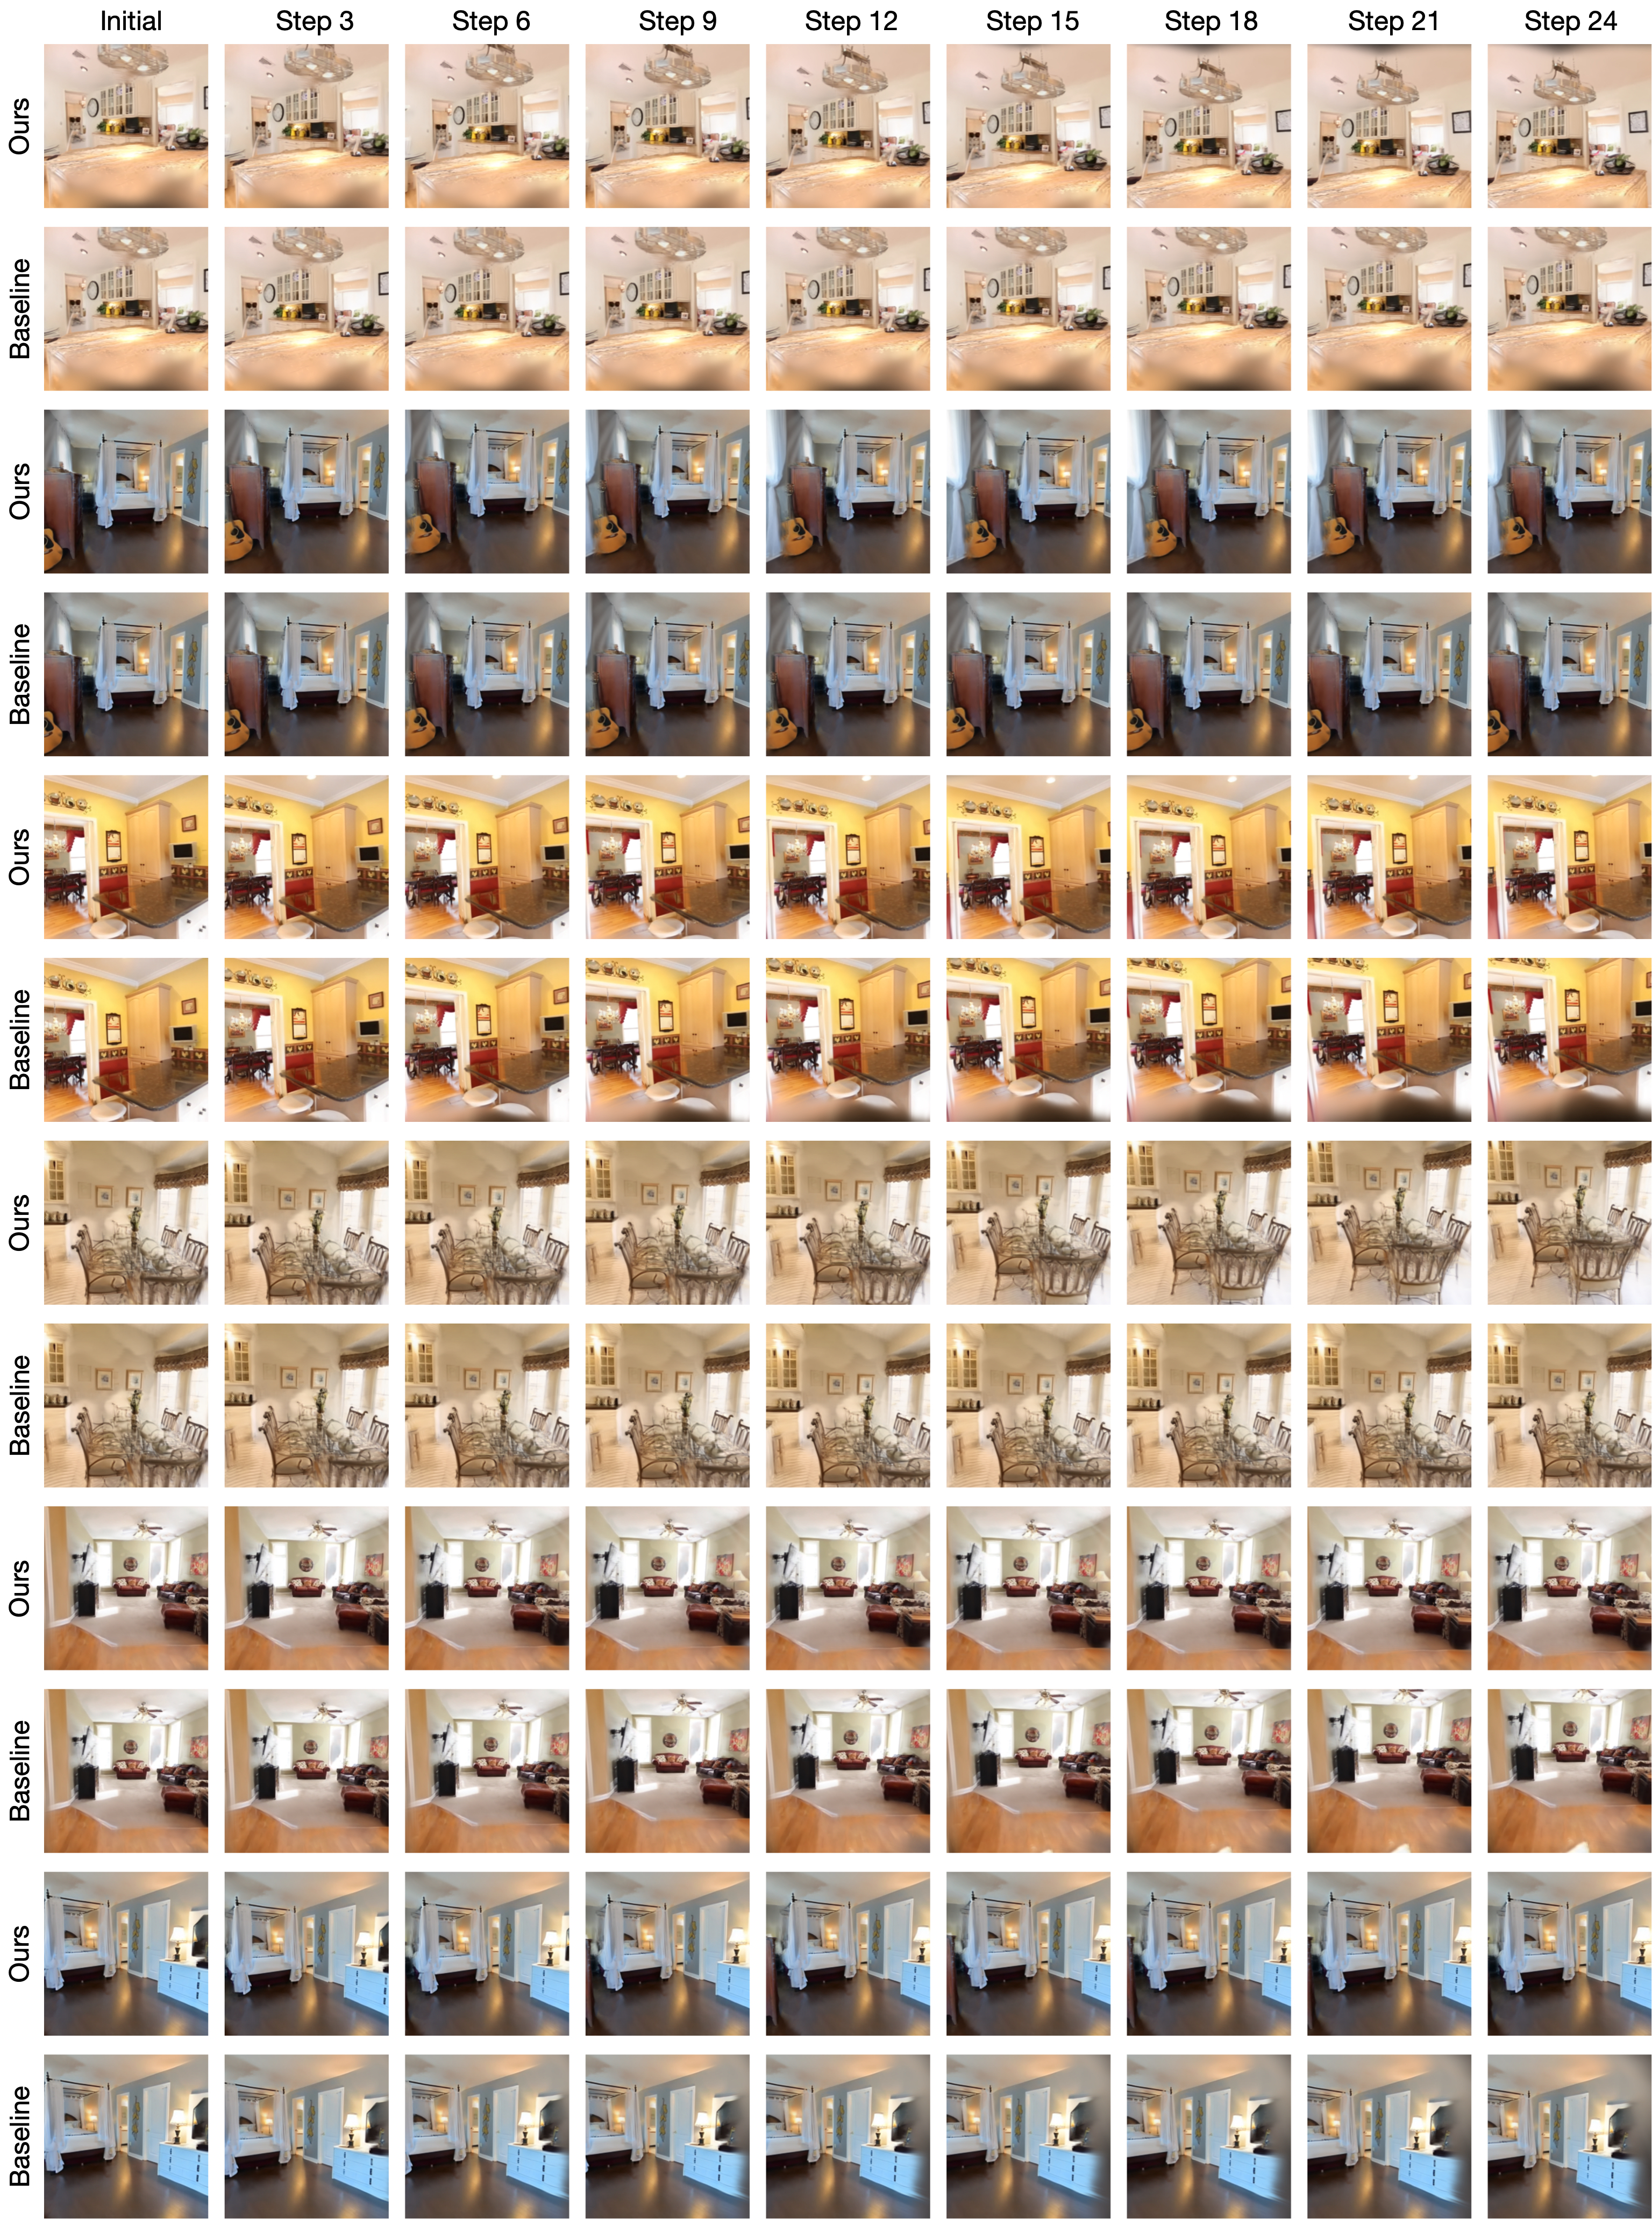
\includegraphics[width=0.92\linewidth]{figs/sup_grad_vertical.jpg}
    \caption{Additional gradient ascent results. Zoom in for a closer look.}
    \label{fig:sup_grad}
\end{figure*}

\section{Aesthetic Field Gradient Optimization}
We present additional results comparing gradient ascent optimization using the baseline approach and our method. As shown in~\cref{fig:sup_grad}, our method consistently converges toward more aesthetically pleasing viewpoints, whereas the baseline approach often fails to make meaningful progress and can sometimes degenerate.

\begin{table}[t]
\small
  \centering
  \begin{tabular}{l| c c  c c  c}
    \toprule
    & $S=4$& $S=8$& $S=16$& $S=32$\\
    \midrule
    $N=4$ & 1.98 & 2.00 & 1.98 & 1.98  \\
    $N=8$ & 1.98 & 1.94 & 2.03 & 2.02 \\
    $N=16$ & 2.01 & 2.00 & 2.02 & 2.04  \\
    $N=32$ & 2.02 & 2.03 & 2.04 & 2.06  \\
    \bottomrule
  \end{tabular}
  \caption{Ablation of the sampling configuration of search stage 1 on novel view aesthetic prediction. $S$ denotes the number of samples along each segment of the interpolated input-view trajectory, and $N$ denotes the number of neighboring viewpoints sampled around each segment-sample. All experiments use 4 input views on RE10k~\cite{re10k}, and the aesthetic quality is measured by VEN~\cite{wei2018good}.}
  \label{tab:sup_ablate}
\end{table}

\section{Ablations}
We provide additional ablation experiments of the Stage 1 search configuration, focusing on two parameters: the number of samples along each input-view segment ($S$) and the number of neighbors further drawn around each segment sample ($N$). The total number of candidate viewpoints is approximately proportional to $S\times N$. We measure the aesthetic qualities of final suggestions via VEN~\cite{wei2018good}. As shown in ~\cref{tab:sup_ablate}, our method remains stable across a wide range of sampling densities, while generally achieving better performance with more samples. We adopt $S=16$ and $N=8$ as our default configuration, as this setting offers a good balance between suggestion quality and total number of samples being evaluated.

% \begin{itemize}
% \item The supplementary can back-reference sections of the main paper, for example, we can refer to \cref{sec:intro};
% \item The main paper can forward reference sub-sections within the supplementary explicitly (e.g. referring to a particular experiment); 
% \item When submitted to arXiv, the supplementary will already included at the end of the paper.
% \end{itemize}
% 
% To split the supplementary pages from the main paper, you can use \href{https://support.apple.com/en-ca/guide/preview/prvw11793/mac#:~:text=Delete%20a%20page%20from%20a,or%20choose%20Edit%20%3E%20Delete).}{Preview (on macOS)}, \href{https://www.adobe.com/acrobat/how-to/delete-pages-from-pdf.html#:~:text=Choose%20%E2%80%9CTools%E2%80%9D%20%3E%20%E2%80%9COrganize,or%20pages%20from%20the%20file.}{Adobe Acrobat} (on all OSs), as well as \href{https://superuser.com/questions/517986/is-it-possible-to-delete-some-pages-of-a-pdf-document}{command line tools}.